\documentclass[a4paper, 10pt]{article}

\usepackage{hyperref}
\usepackage[utf8]{inputenc}
\usepackage[french]{babel}
\usepackage{eurosym} % \oe{} ...
\usepackage{graphicx}
\usepackage[T1]{fontenc}
\usepackage{geometry}
\usepackage{fancyhdr}
\usepackage{lastpage}
\usepackage{paralist}
\usepackage{listings}
\usepackage{color}
\usepackage{amsmath}

\lstset{language=Java, frame=shadowbox, rulesepcolor=\color{black}}

\geometry{hmargin=1.5cm, vmargin=2cm }
\pagestyle{fancy}
\setlength\parindent{0pt}

\lhead{\'Ecole des Mines de Douai -- Mineur MAD} \lfoot{G.L.}
\rhead{TD/TP 01 - Décisions sous incertitude}
\rfoot{Page : \thepage/\pageref{LastPage}}
\cfoot{} \chead{}

\newcounter{QQ}

\newcommand{\question}[1]{ \medskip \sffamily \textsc{\textbf{\large Question \stepcounter{QQ} \arabic{QQ}} \emph{\small(#1)}} : }

\begin{document}
\author{\'Ecole des Mines de Douai -- FI 2A}
\date{}
\title{\Large{\textbf{Exam - Décisions sous incertitude: Troll}}}
\maketitle
\thispagestyle{fancy}

% \section*{Nom(s) et prénom(s): \_\_\_\_\_\_\_\_\_\_\_\_\_\_ $\quad$ \_\_\_\_\_\_\_\_\_\_\_\_\_\_}

% \bigskip

% Le barème est indicatif et sera ajusté lors de la correction.

\section*{Retro-engineering}

Vous êtes en possession du script suivant décrivant le comportement d'un Troll dans un jeu vidéo et vous souhaitez comprendre ce comportement.

\begin{lstlisting}[caption={Script}]
  String behavior( int [] s )
  if( s[0] == 1 )
  {
    if( s[1] == 1 )
      return "run away";
    else
      return "attack";
  }
  else
  {
    if( s[1] < 3 )
      return "sleep";
    else
    {
      if( s[2] == 0 )
        return "explore";
      else
        return "socialize";
    }
  }
\end{lstlisting}

\question{3 points} Construire l'arbre de décision correspondant au comportement du Troll.

\question{1.5 points} Énumérer les variables et les domaines de variation possibles pour ce comportement.

\question{0.5 point} Quel est la taille de l'espace d'état que couvre cet arbre de décision ?

\question{1 point} Qu'elle est l'action retournée par l'état $[1,\ 2,\ 1]$ ?

\question{1 point} Combien d'états sont représentés par la feuille pointée par l'état $[1,\ 2,\ 1]$ ? (calculs et résulta)
  
\question{1 point} Proposer des noms cohérents pour chacune des variables d'état avec une courte justification. 


\section{Probabilities on attack outcome }
  
  On souhaite modéliser un combat entre un Troll et un Chevalier (Knight) de façon à améliorer le comportement du Troll.
  Le Troll et le Chevalier ont tous les deux un niveau de vie (health) débutant à $3$ et descendant jusqu'à $0$ ($3$: healthy ; $2$: hurt ; $1$: dying ; $0$: dead).
  Pendant une attaque d'un Troll, le Troll peut potentiellement toucher le chevalier et réduire sa vie avec de $1$ à $3$ dommages.
  Dans des conditions normales, le Troll a $0.1$ chance de faire $1$ dommage, $0.4$ chance de faire $2$ dommages et  $0.2$ chance de faire $3$ dommages, autrement, le chevalier esquive l'attaque.
  Si la vie du Troll est diminuée (hurt, dying), ses chances de faire des dommages sont réduites de la moitié de leur valeur pour chaque point de vie perdu par le Troll.
  De plus, le chevalier possède potentiellement un bouclier (shield), dans ce cas, les dommages qu'il reçoit sont diminués de $1$.

\question{2 points}
  Proposer un réseau Bayesian permettant de calculer les probabilités sur les dommages causés par le Troll lors d'une attaque.
  
\question{2 points}
  Donner le tableau des probabilités conditionnelles attachées au n\oe{}ud représentant les dommages infligés par le Troll.

\question{1 point}
  En considérant que le Troll est en pleine forme (healthy) et que la moitié des Chevaliers rencontrés utilise un bouclier, quelle est la probabilité que le Troll tue le chevalier à la première attaque ? (calculs sur la base du réseau Bayesien proposé et résultat)
  
\question{2 points}
  Un combat entre un Troll et un Chevalier est composé par plusieurs attaques du Troll où le chevalier pourra contre-attaquer s'il est en vie et s'il n'a subi aucun dommage (après une esquive ou si le bouclier a absorbé tous les dommages).
  Une contre-attaque fait $1$ dommage avec une probabilité de $0.5$ et $2$ dommages avec une probabilité de $0.2$ quelque soit l'état de santé du Troll ou du Chevalier.
  Enfin, les dommages causés par le Chevalier sont augmentés de $1$ s'il n'a pas de bouclier (lui permettant d'être mieux armé).
  Proposer un nouveau réseau Bayesien modélisant l'évolution des points de vie du Troll et du Chevalier.

\question{1 point} Quel est le nom de ce type de réseau bayésien ?

\question{3 points}
  Implémenté en Java la fonction qui retourne les probabilités sur l'évolution des points de vie du Troll en s'appuyant sur le réseau Bayesien proposé.
  La fonction prend autant de paramètres qu'il y a de variables utiles au calcul de ces probabilités (sous forme d'entiers avec des noms appropriés) et retourne un tableau de $4$ probabilité (une pour chacune des $4$ niveaux de vie possibles).
  Exemple de signature de fonction attendue (avec \emph{nva} pour nom de variable approprié) : 
  $$ \text{\emph{ double [] trollHealthEvolution( int nva1,  int nva2,  int nva3, [...] ) }} $$

\section{Markov Decision Process}
  
  Basé sur le réseau Bayesien modélisant un combat, on propose de développer un processus de décision Markovien pour modéliser un combat entre un Troll et un Chevalier utilisant un bouclier.
  Les états sont simplement construits sur les points de vie du Troll et du Chevalier (vivant) et avec trois états supplémentaires modélisant le fait que le Troll ou le Chevalier est mort et la fin du combat.
  La décision pour le Troll consiste à attaquer (attack) ou fuir (run away).
  L'action ``run away'' termine systématiquement dans l'état \emph{End} fin du combat, avec une probabilité à $1.0$.
  Les transitions de l'action ``attack'' sont modélisées par la figure ci après. 
  Le modèle est composé de $12$ état et $2$ actions.
  La fonction de récompense représente le plaisir qu'a le Troll d'attaquer et tuer du Chevalier.
  
  $$ r(s, a)= \left\{
  \begin{array}{r l}
      -10  & \text{if Troll is dead} \\
      8    & \text{if Knight is dead} \\
      0    & \text{if combat is ended} \\
      2    & \text{if Troll is attacking (combat not ended and Troll or Knight not dead)} \\
      0    & \text{if Troll is running away}
   \end{array}
   \right.$$

   \begin{figure}[!b]
    \centering
    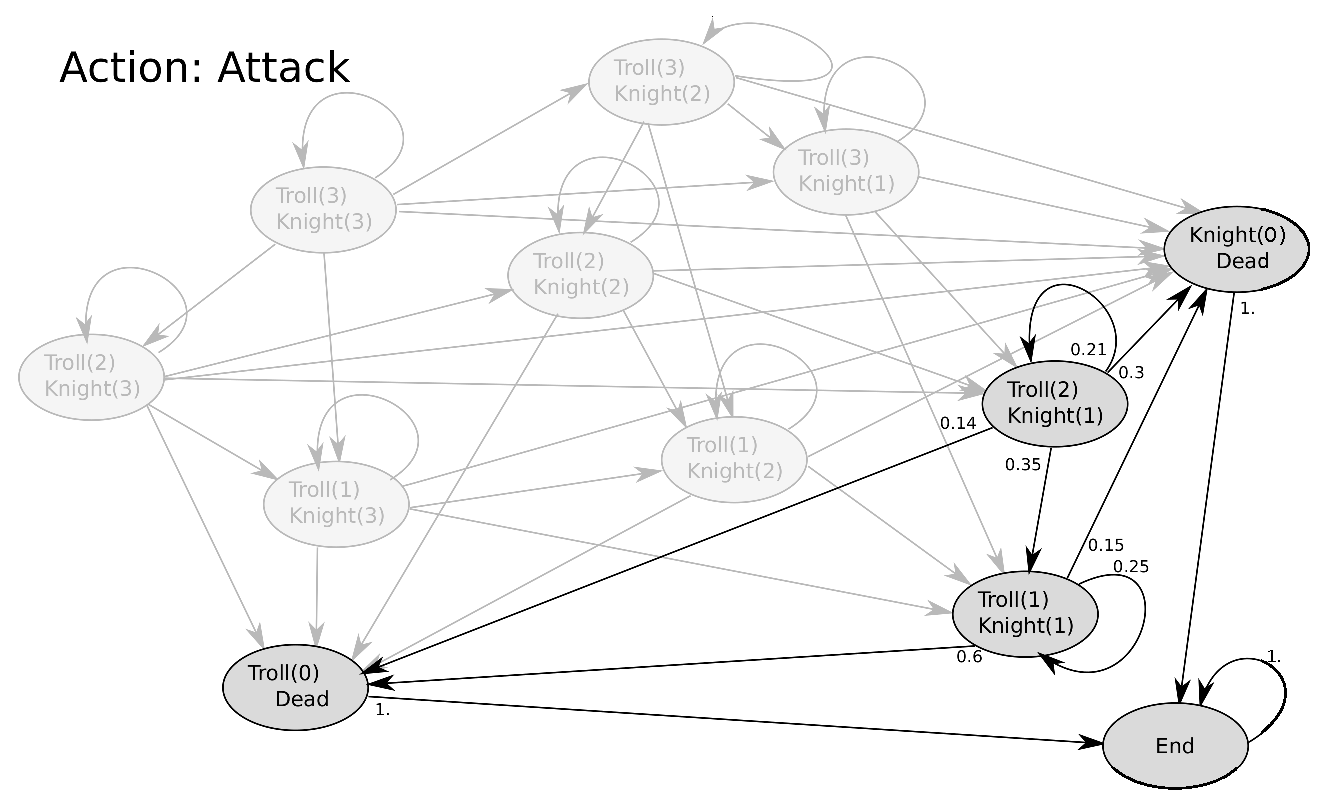
\includegraphics[width=0.6\textwidth]{fig/Attacking}
    \caption{Fonction de transition pour l'action ``attack'' (focalisé sur les états ciblés par les questions 13 et 14)}
   \end{figure}

\question{1 point}
  En considérant l'équation de Bellman, quelle est la meilleure action et sa valeur associée au pas de temps $t=1$ pour chacun de ces $5$ états:
  (\emph{End} ; \emph{Troll(0)} ; \emph{Knight(0)}
  \emph{Troll(2)-Knight(1)} ; \emph{Troll(1)-Knight(1)}.
  $$ \text{Équation de Bellman :} \qquad V_t(s)= \max_{a}\left(r(s,\ a) + \sum_{s'\in S} t(s,\ a,\ s') V_{t-1}(s') \right) \quad \text{avec} \quad V_0(s)= 0  $$
\question{2 points} Même question, pour le pas de temps $t=2$.



\end{document}